% Generated on 2026-07-20 from the zero-shot v9 + direction-fallback run.
% Requires: \usepackage{booktabs} and \usepackage{graphicx}
\begin{table}[t]
  \centering
  \caption{MemQ v9 with direction fallback. GrailQA uses the labelled v1.0
  development split; no GrailQA example was used for fine-tuning. EHR and
  GoldGED are aggregate reconstruction metrics; H@1 and Macro-F1 are answer
  metrics.}
  \label{tab:memq-v9-all-datasets}
  \begin{tabular}{llrrrr}
    \toprule
    Dataset & evaluated split & EHR $\uparrow$ & GoldGED $\downarrow$ & H@1 $\uparrow$ & Macro-F1 $\uparrow$ \\
    \midrule
    WebQSP & test ($n=1{,}626$) & 0.502 & 1.784 & 0.822 & 0.823 \\
    CWQ & test ($n=3{,}273$) & 0.498 & 2.648 & 0.723 & 0.738 \\
    GrailQA & dev ($n=4{,}970$) & 0.008 & 3.434 & 0.018 & 0.018 \\
    GrailQA++ & -- & \multicolumn{4}{c}{No official labelled release was available for evaluation.} \\
    \bottomrule
  \end{tabular}
\end{table}

\begin{figure*}[t]
  \centering
  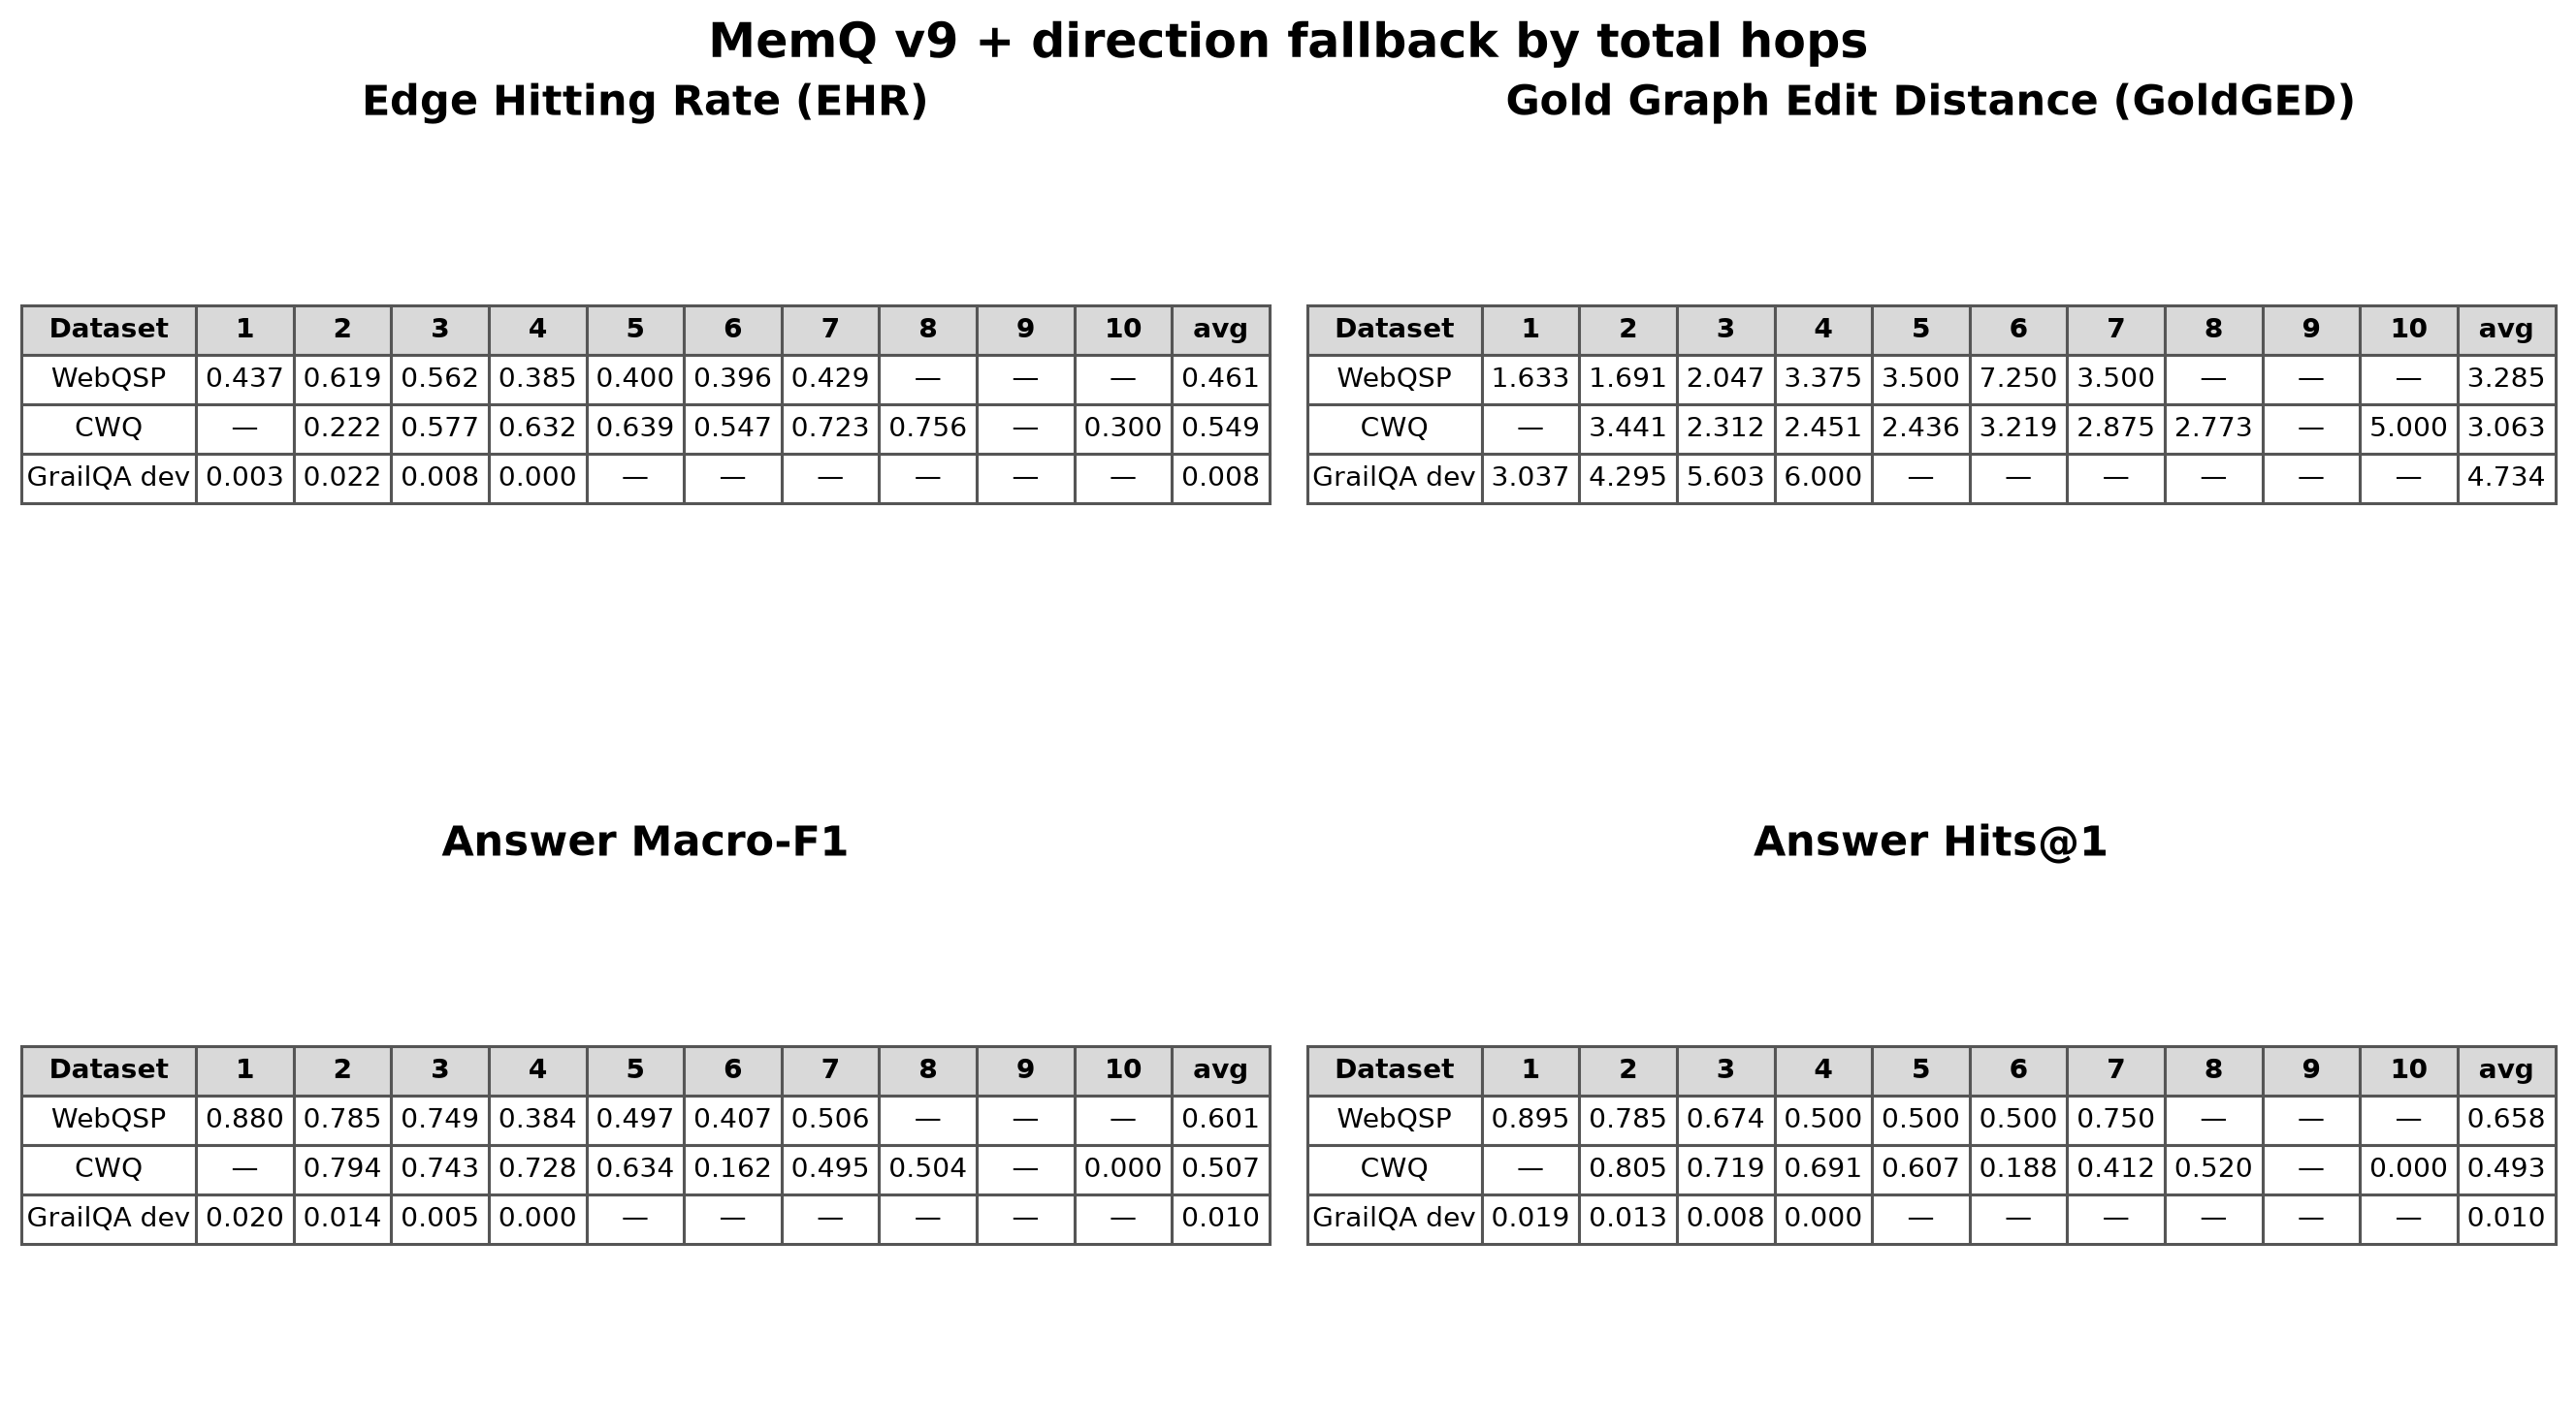
\includegraphics[width=\textwidth]{figures/memq_v9_hop_metrics.png}
  \caption{Hop-wise breakdown for the evaluated datasets. The values are
  means within each total-hop group; a dash denotes that the split has no
  examples in that group.}
  \label{fig:memq-v9-hop-metrics}
\end{figure*}
